\documentclass[12pt,a4paper,titlepage]{article}
\usepackage[utf8]{inputenc}
\usepackage{polski}
\usepackage{listings}
\usepackage{graphicx}
\usepackage{xcolor}
\usepackage{minted}
\usepackage{amsmath}
\usepackage{caption}
\usepackage{hyperref}

\renewcommand\listoflistingscaption{Spis listingów}

\setminted{
    autogobble,
    breaklines,
    framerule=1pt,
    framesep=10pt
}

\newenvironment{longlisting}{}{}

\makeatletter
\newcommand{\linia}{\rule{\linewidth}{0.4mm}}
\renewcommand{\maketitle}{\begin{titlepage}
    \vspace*{1cm}
    \begin{center}\small
    Politechnika Wrocławska\\
    Wydział Elektroniki\\
    Bezpieczeństwo Systemów i Usług Informatycznych 2
    \end{center}
    \vspace{3cm}
    \noindent\linia
    \begin{center}
      \LARGE \textsc{\@title}
         \end{center}
     \linia
    \vspace{0.5cm}
    \begin{flushright}
    \begin{minipage}{7cm}
    \textit{\small Autor:}\\
    \normalsize \textsc{\@author} \par
    \end{minipage}
    \vspace{5cm}

     {\small wtorek, 11\textsuperscript{15}-14\textsuperscript{00} TN}\\
        Mgr inż. Przemysław Świercz
     \end{flushright}
    \vspace*{\stretch{6}}
    \begin{center}
    \@date
    \end{center}
  \end{titlepage}%
}
\makeatother
\author{Justyna Skalska, 225942}
\title{Sprawozdanie nr 5\\
(Exploitme)}

\begin{document}

\maketitle

\tableofcontents 
\newpage
\listoflistings
\newpage
\listoffigures
\newpage

\section{Omówienie tematu}
\subsection{Wstęp}
Naszym zadaniem podczas laboratorium było rozwiązanie zagadki typu exploitme. Dostaliśmy aplikację, na której należało przeprowadzić atak polegający przepełnienia bufora. Polegało to na zmianie parametrów oraz adresu powrotu funkcji. Wykorzystaliśmy do tego GDB (GNU Debugger) oraz skrypty stworzone w języku Perl.

\subsection{Przepełnienie bufora}
Otrzymany przez nas program zawierał funkcję \mintinline{bash}{validate}, gdzie wykorzystano funkcję \mintinline{c}{strcpy}. Nie sprawdza ona długości kopiowanych znaków, przez co program może być podatny na ataki przepełnienia bufora (ang. \textit{buffer overflow}), jeśli programista nie zapewnił wcześniejszego sprawdzenia długości. Ataki te polegają na zapisaniu do wyznaczonego obszaru pamięci (bufora) większej ilości danych niż zarezerwował na ten cel programista. Taka sytuacja prowadzi do zamazania danych znajdujących się w pamięci bezpośrednio za buforem, a w rezultacie do błędnego działania programu. Gdy dane, które wpisywane są do bufora, podlegają kontroli osoby o potencjalnie wrogich intencjach, może dojść do nadpisania struktur kontrolnych programu w taki sposób, by zaczął on wykonywać operacje określone przez atakującego.~\cite{buffer-overflow}
\newline\newline
W naszej przykładowej aplikacji będziemy nadpisywać adres powrotu funkcji. Rysunek \ref{fig:stack} przedstawia wygląd stosu w architekturze x86–64~\cite{stack}. Widać na nim, że adres powrotu znajduje się ponad argumentami funkcji. Aby przepełnić bufor i nadpisać adres powrotu należy sprawdzić jaka wielkość danych powoduje błąd naruszenia pamięci podczas działania programu.

\begin{figure}[H]
\centering
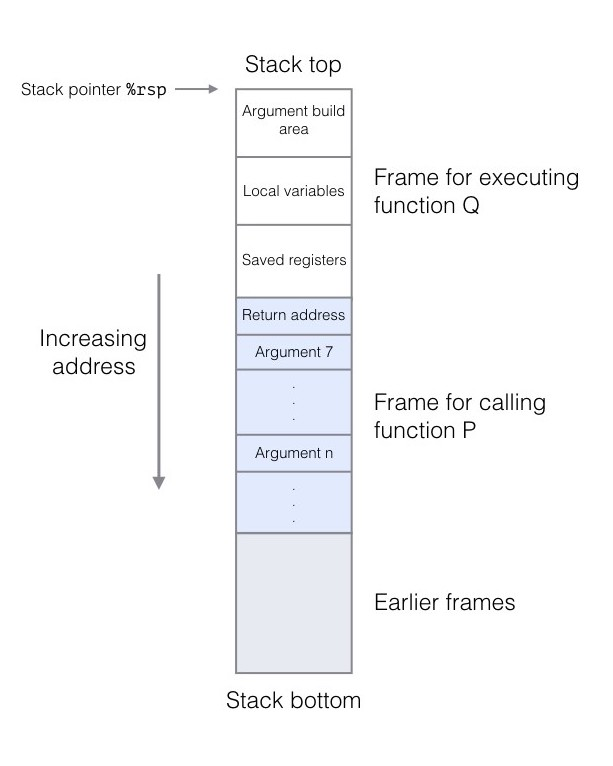
\includegraphics[width=10cm]{images/stack.jpeg}
\caption{Ogólna struktura ramki stosu w architekturze x86–64 dla funkcji P, która wywołuje funkcję Q.}
\label{fig:stack}
\end{figure}

\subsection{Shellcode}
Shellcode (pl. \textit{kod powłoki}) to zestaw instrukcji wstrzykiwanych, a następnie wykonywanych przez wykorzystywany program. Shellcode służy do bezpośredniej manipulacji rejestrami i funkcjonalności wykorzystywanego programu. Piszemy je, ponieważ chcemy, aby program docelowy działał w sposób inny niż zamierzony przez projektanta. Jednym ze sposobów manipulowania programem jest zmuszenie go do wykonania wywołania systemowego lub syscall. Wywołania systemowe w Linuksie są realizowane przez przerwania programowe i wywoływane są instrukcją zaczynającą się przez 0x80. Kiedy kod 0x80 jest wykonywany przez program uruchomiony przez użytkownika, CPU przełącza się w tryb jądra i wykonuje funkcję syscall.~\cite{shellcode}

\begin{listing}[H]
\caption{Przykładowy shellcode składający się z różnych instrukcji.}
\begin{minted}{c}
char shellcode[]=          
    "\x31\xc0"      // xorl    %eax,%eax
    "\x31\xdb"      // xorl    %ebx,%ebx
    "\x31\xc9"      // xorl    %ecx,%ecx
    "\xb0\x46"      // movl    %al,$0x46
    "\xcd\x80"      // int     $0x80
    "\x50"          // pushl   %eax
    "\x68""/ash"    // pushl   $0x6873612f
    "\x68""/bin"    // pushl   $0x6e69622f
    "\x89\xe3"      // movl    %esp,%ebx
    "\x50"          // pushl   %eax
    "\x53"          // pushl   %ebx
    "\x89\xe1"      // movl    %ecx,%esp
    "\xb0\x0b"      // movb    %al,$0x0b
    "\xcd\x80"      // int     $0x80
;
\end{minted}
\end{listing}

\subsection{Little endian}
\noindent\begin{minipage}{0.6\textwidth}
Little endian to forma zapisu danych, w której najmniej znaczący bajt (zwany też dolnym bajtem, z ang. \textit{low-order byte}) umieszczony jest jako pierwszy. Kolejne bajty następują w kolejności rosnącego znaczenia. Procesory, które używają formy little endian, to między innymi wszystkie z rodziny x86, DEC VAX.~\cite{little-endian} Na rysunku~\ref{fig:little-endian} pokazany jest przykład zapisywania w pamięci liczby całkowitej \mintinline{bash}{0A0B0C0D}.

\end{minipage}
\hfill
\noindent\begin{minipage}{0.35\textwidth}
\begin{figure}[H]
\centering
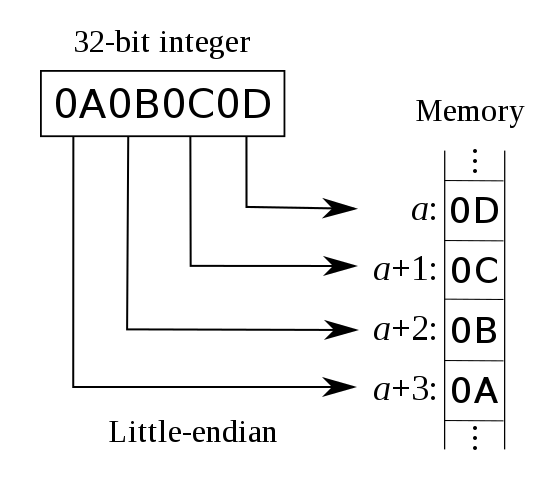
\includegraphics[width=\textwidth]{images/little-endian.png}
\caption{Little endian.}
\label{fig:little-endian}
\end{figure}
\end{minipage}

\newpage
\section{Omówienie rozwiązania}
\subsection{Przepełnienie bufora}
Pierwsza część zadania polegała na znalezieniu najmniejszej liczby znaków, która powodowała przepełnienie bufora. Aplikacja przyjmowała jeden argument będący ciągiem znaków. Wystarczyło odpalić program podając mu różną długość argumentu. Moje pierwsze podejście używało podanej niżej komendy, której argument miał 22 znaki.
% \begin{listing}[H]
% % \caption{Składnia komendy odpalającej plik w debuggerze GDB z argumentami.}
% \begin{minted}{bash}
% ./exploitme shshdfshdfhdfhdshdfhsd
% \end{minted}
% \end{listing}
\newline\newline
\mintinline{bash}{./exploitme shshdfshdfhdfhdshdfhsd}
\newline

Po kilku próbach okazało się, że najmniejsza liczba znaków, dla której aplikacja nie kończy się błędem wynosi 53. Przy użyciu 54 znaków następuje naruszenie ochrony pamięci. Wysłany przez mnie ciąg znaków zawierał także znak końca tekstu, którego nie widać jawnie podczas wpisywania ciągu. Wynika z tego, że maksymalna liczba bajtów, która nie powoduje naruszenia ochrony pamięci wynosi 54.
Następnie dowiedzieliśmy się, że można odpalać GDB podając argumenty do debugowanego programu. Składnia wygląda następująco:
\newline\newline
\mintinline{bash}{gdb --args <plik> [args]}
\newline

Dzięki użyciu GDB można w łatwy sposób podać argumenty do programu korzystając z języka Perl. Poniżej znajduje się przykładowa komenda wywołująca kod Perla, który generuje ciąg złożony z 53 jedynek.
\begin{listing}[H]
\caption{Wywołanie pliku z argumentami w GDB}
\begin{minted}{bash}
gdb --args exploitme `perl -e 'print "1"x53'`
\end{minted}
\end{listing}

\subsection{Wywołanie funkcji programu}
Kolejnym zadaniem na laboratorium było wywołanie dwóch funkcji zaimplementowanych w programie. Ich adresy można było odczytać z kodu assemblerowego:
\begin{itemize}
    \item \mintinline{bash}{0x080485d7} - destroy\_world,
    \item \mintinline{bash}{0x080486ce} - reboot
\end{itemize}

Należało wykorzystać do tego wcześniej nabytą wiedzę o tym, że 55 bajtów powoduje błąd naruszenia pamięci. Można z tego wywnioskować, że nadpisujemy adres powrotu funkcji. Parametry wywołania aplikacji w GDB należało podać w następującej kolejności:
\newline\newline
\mintinline{bash}{<offset><return address>}
\newline

Wyposażeni w tę wiedzę mogliśmy spróbować zapisać tam adres, w którym zaczyna się wywołanie pożądanej przez nas funkcji destroy\_world lub reboot. Przedstawione wcześniej adresy musieliśmy podać jako argument wywołania w formacie little endian.


\begin{listing}[H]
\caption{Wywołanie funkcji destroy\_world}
\begin{minted}{bash}
gdb --args exploitme `perl -e 'print "1"x54 . "\xD7\x85\x04\x08"'`
\end{minted}
\end{listing}

\begin{listing}[H]
\caption{Wywołanie funkcji reboot}
\begin{minted}{bash}
gdb --args exploitme `perl -e 'print "1"x54 . "\xce\x86\x04\x08"'`
\end{minted}
\end{listing}

\subsection{Wywołanie funkcji systemowej}
Ostatnim etapem było wywołanie funkcji systemowej, dzięki której otworzy nam się Bash. Po wyjściu z niego komendą \mintinline{bash}{quit} aplikacja miała zakończyć się bez błędu, z kodem 0x12.\newline\newline
Przydatne w tej części adresy:
\begin{itemize}
    \item \mintinline{bash}{0x08048454} - wywołanie systemowe (ang. \textit{system call}) 
    \item \mintinline{bash}{0x080487d0} - Bash (powłoka systemu),
    \item \mintinline{bash}{0x804084d4} - wywołanie systemowe exit.
\end{itemize}

Pierwszym krokiem było wywołanie funkcji systemowej z parametrem wywołującym powłokę systemu (Bash). Parametry wywołania aplikacji w GDB należało podać w następującej kolejności:
\newline\newline
\mintinline{bash}{<offset><system><system return><system parameter>}
\newline

Nasz offset nadal wynosi 54 znaki. Tuż po nim znajduje się adres funkcji systemowej, której parametr wywołania podajemy jako ostatni. Jest nim podany wyżej adres powłoki systemu. Między nimi znajduje się adres powrotu po wykonaniu podanego wcześniej wywołania. W tym miejscu podajemy adres wywołania systemowego \mintinline{bash}{exit}.

\begin{listing}[H]
\caption{Wywołanie powłoki systemowej}
\begin{minted}{bash}
gdb --args exploitme `perl -e 'print "1"x54 . "\x54\x84\x04\x08" . "\xd4\x84\x04\x08" . "\xd0\x87\x04\x08"'`
\end{minted}
\end{listing}

Ostatnim krokiem było zmodyfikowanie wcześniej stworzonych parametrów, tak aby aplikacja po wywołaniu Basha zamknęła się bez błędu z kodem 0x12. Parametry wywołania aplikacji w GDB należało podać w następującej kolejności:
\newline\newline
\mintinline{bash}{<offset><system><system return><system parameter><exit param>}
\newline

Pojawił się tu nowy fragment odnoszący się do parametru wywołania systemowego \mintinline{bash}{exit}. Jako ten parametr podajemy oczekiwany przez nas kod.

\begin{listing}[H]
\caption{Wywołanie powłoki systemowej i zakończenie programu z kodem 0x12}
\begin{minted}{bash}
gdb --args exploitme `perl -e 'print "1"x54 . "\x54\x84\x04\x08" . "\xd4\x84\x04\x08" . "\xd0\x87\x04\x08" . "\x12"'`
\end{minted}
\end{listing}

Po wywołaniu podanej wyżej funkcji spodziewaliśmy się pojawienia kodu 0x12 w zapisie szesnastkowym lub 18 w zapisie dziesiętnym. Zaskoczył nas jednak podany komunikat: \textit{"Program exited with code 022."}. Okazało się, że podany przez nas kod został wypisany w formacie ósemkowym.

\section{Wnioski}
Podczas zajęć udało mi się wykonać wszystkie podpunkty zadania. Dowiedziałam się jak w prosty sposób można wykorzystać błędy programistów do manipulowania aplikacją. Wykorzystanie tej wiedzy w większych programach może być problematyczne, ponieważ wymaga analizowania i zrozumienia kodu assemblera. Trzeba także znać funkcje, które są podatne na ataki. Widać tutaj jak ważną rolę odgrywa wybór odpowiednich funkcji i implementacja warunków wykonania danych fragmentów kodu.

Aby zapobiec tego typu atakom należy brać pod uwagę rozmiar przyjmowanych danych. Trzeba także zwracać uwagę na funkcje, które nie sprawdzają ich wielkości (np. \mintinline{c}{strcpy} w języku C). Powinno się używać bezpieczniejszych odpowiedników takich funkcji (np. \mintinline{c}{strncpy}). 

\newpage
\bibliographystyle{unsrt}
\bibliography{references}

\end{document}